\footnotesize
\tikzstyle{pointer} = [draw, *-triangle 60]
\tikzstyle{tag}     = [rectangle, draw, text width=6em
                      , minimum height=2em, text centered
                      , node distance=4em]
\tikzstyle{payload} = [tag, right, xshift=-0.5pt, text width=3em]

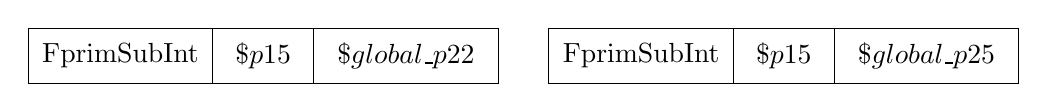
\begin{tikzpicture}[auto]

%% FprimSubIntLeft Node
\node [tag] (FprimSubIntLeft-Tag) {FprimSubInt};
\node [payload] (FprimSubIntLeft-Load1) at (FprimSubIntLeft-Tag.east) {$\$p15$};
\node [payload, text width=6em] (FprimSubIntLeft-Load2) at (FprimSubIntLeft-Load1.east) {$\$global\_p22$};

%% Right subtree

%% FprimSubIntRight Node
\node [tag, right of=FprimSubIntLeft-Load2, xshift=4.5em] (FprimSubIntRight-Tag) {FprimSubInt};
\node [payload] (FprimSubIntRight-Load1) at (FprimSubIntRight-Tag.east) {$\$p15$};
\node [payload, text width=6em] (FprimSubIntRight-Load2) at (FprimSubIntRight-Load1.east) {$\$global\_p25$};

\end{tikzpicture}

